\section{Konzept zur Datenerfassung und - auswertung}
\label{concept}
Ein weiteres wichtiges Thema dieser Arbeit soll es sein, ein erstes Konzept zur automatischen Datenerfassung und - auswertung der nötigen Parameterdaten zu entwickeln. Dieses kann dann als Vorlage für einen Prototypen zur automatischen Einschätzung der Fahrtauglichkeit eines Fahrers vor Fahrtantritt dienen. Der grundlegende Entwurf ist in der Abbildung \ref{fig:conceptfmc} als FMC-Modell dargestellt.

\begin{figure}
	\centering
	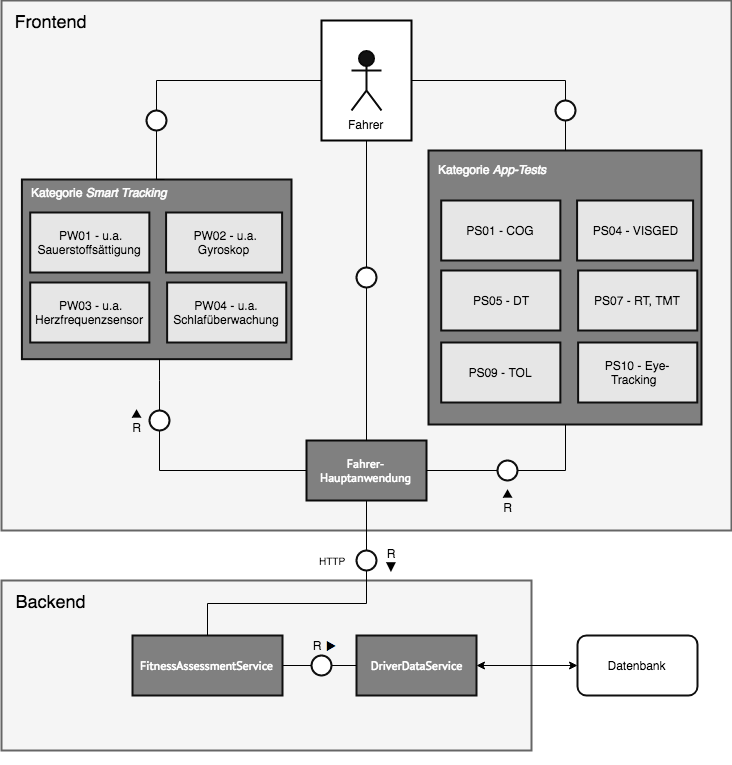
\includegraphics[width=\linewidth]{images/ConceptDriverAssessmentData}
	\caption[Caption for concept]{FMC-Modell der grundlegenden Anwendung}
	\label{fig:conceptfmc}
\end{figure}